%!TEX root = main.tex

\subsubsection{Large-scale Evaluation}
\label{sec:eval}

We evaluate the performance and properties of \cf 's interference management in large scale networks using the ns3 simulator ~\cite{ns3url}. 
Simulations are parametrized based on the experiments in the previous section, (the control channel interference and imperfect CQI reporting).
Overall, the evaluation examines a set of static and dynamic traffic scenarios along three dimensions.\\[2pt]
\noindent $\bullet$ \emph{MAC effects on throughput and coverage} in presence of interference, and comparison against LTE and \wf. \\[2pt]
\noindent $\bullet$ \emph{Application-level performance} by measuring the page download times of a web-like workload. \\[2pt]
\noindent $\bullet$ \emph{Distributed subchannel selection}. We evaluate \cf's resource allocation 
against a centralized, oracle-based state-of-the-art OFDMA resource isolation scheme~\cite{fermi}.\\


\begin{figure*}[htb!]
  %\hfill
  \begin{minipage}{0.33\textwidth}
    \centering
    (a)
    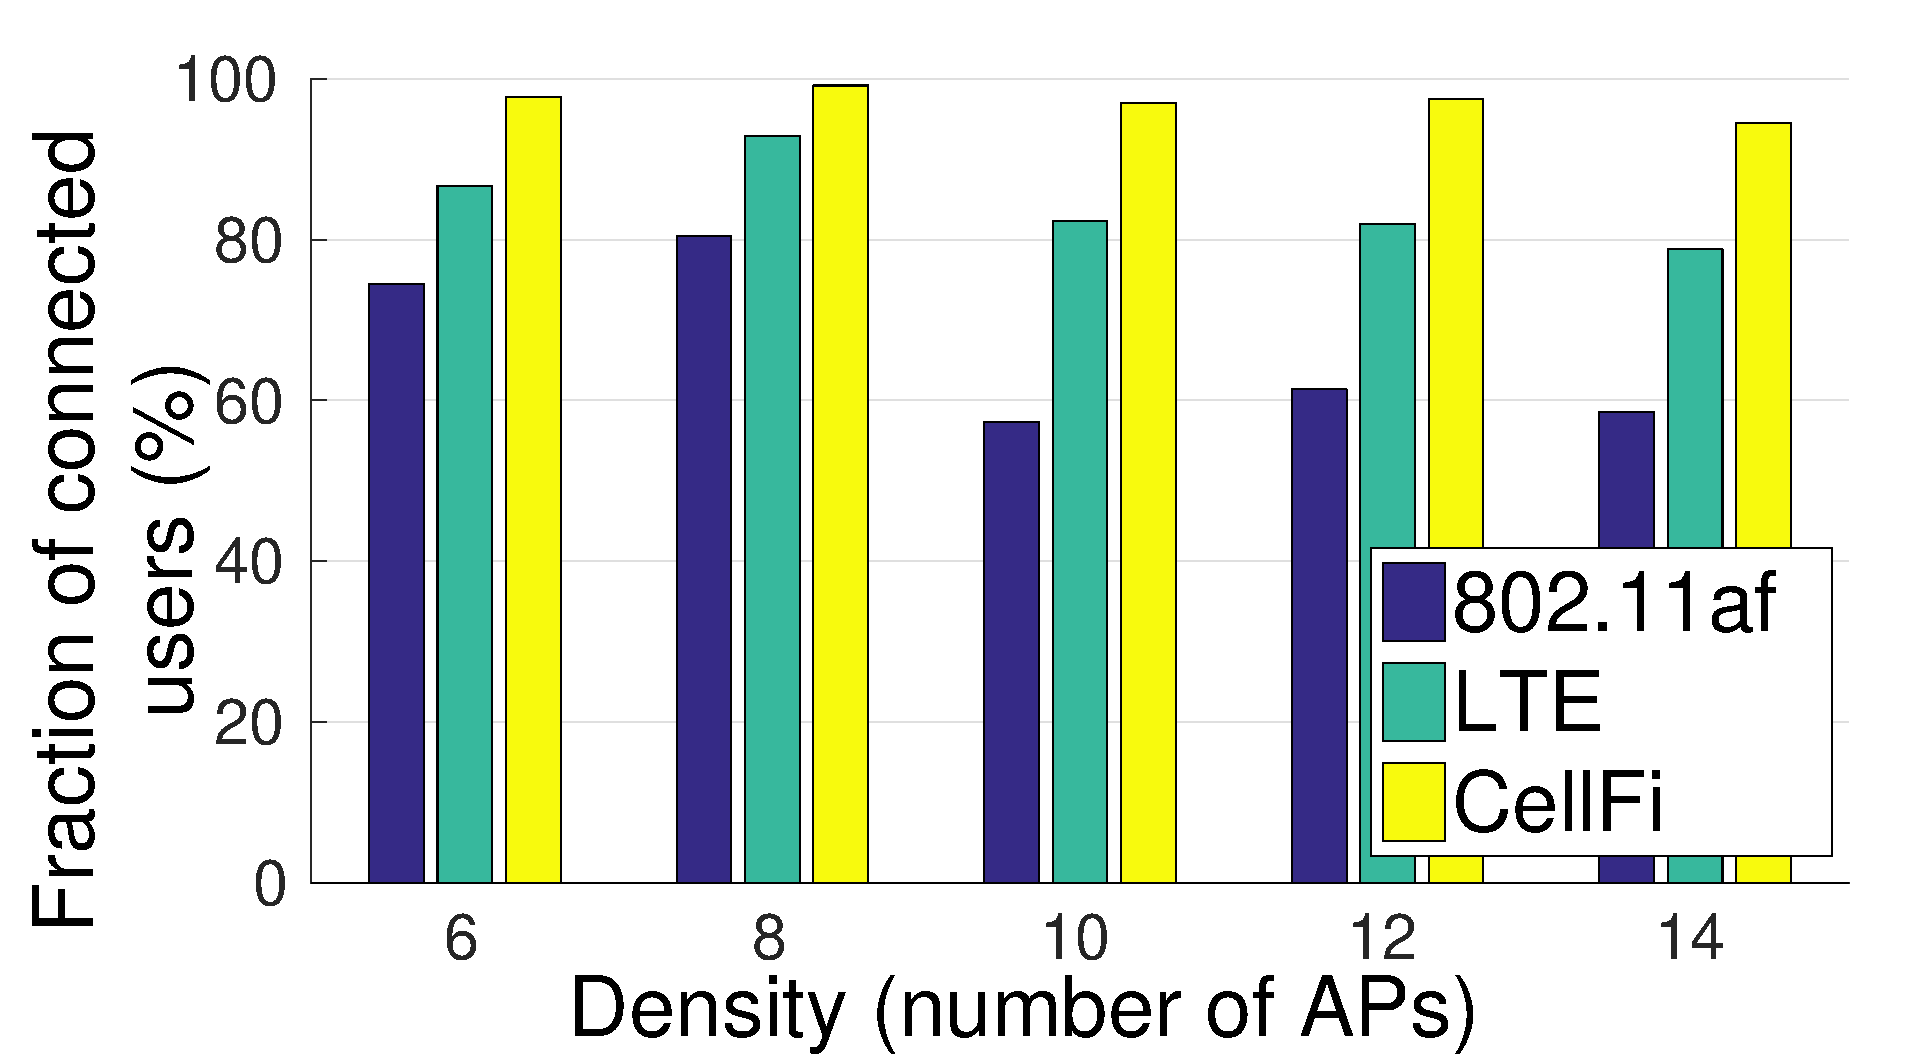
\includegraphics[width=\textwidth]{./figs/density-crop}
  \end{minipage}
  \hspace{1pt}
  \begin{minipage}{0.33\textwidth}
    \centering
    (b)
    \vfill
    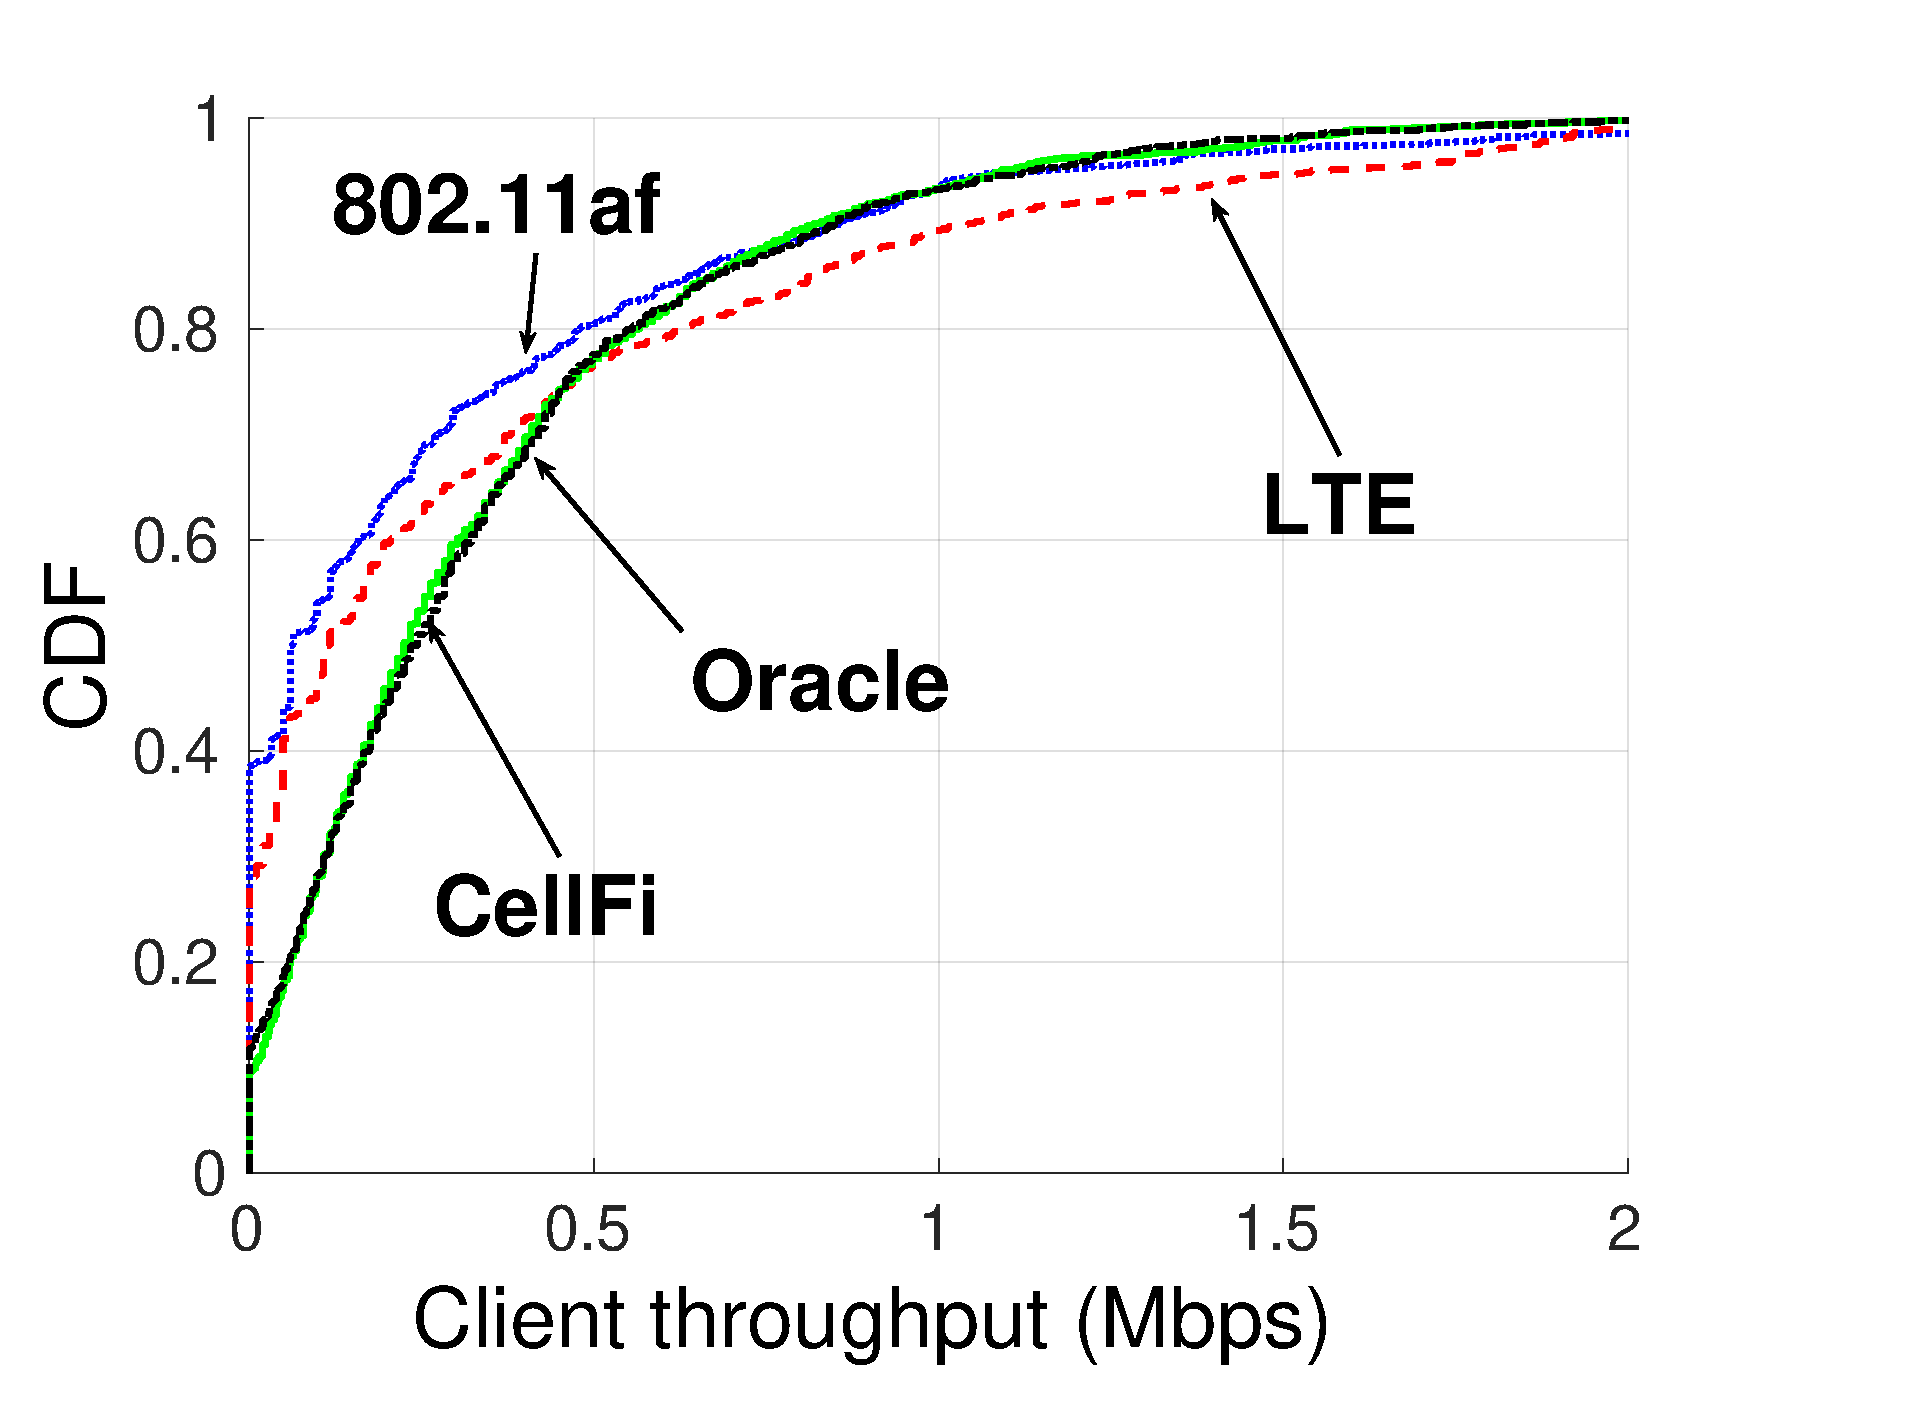
\includegraphics[width=\textwidth, height=0.55\columnwidth]{./figs/cli-crop}
  \end{minipage}
  \begin{minipage}{0.33\textwidth}
    \centering
    (c)
    \vfill
  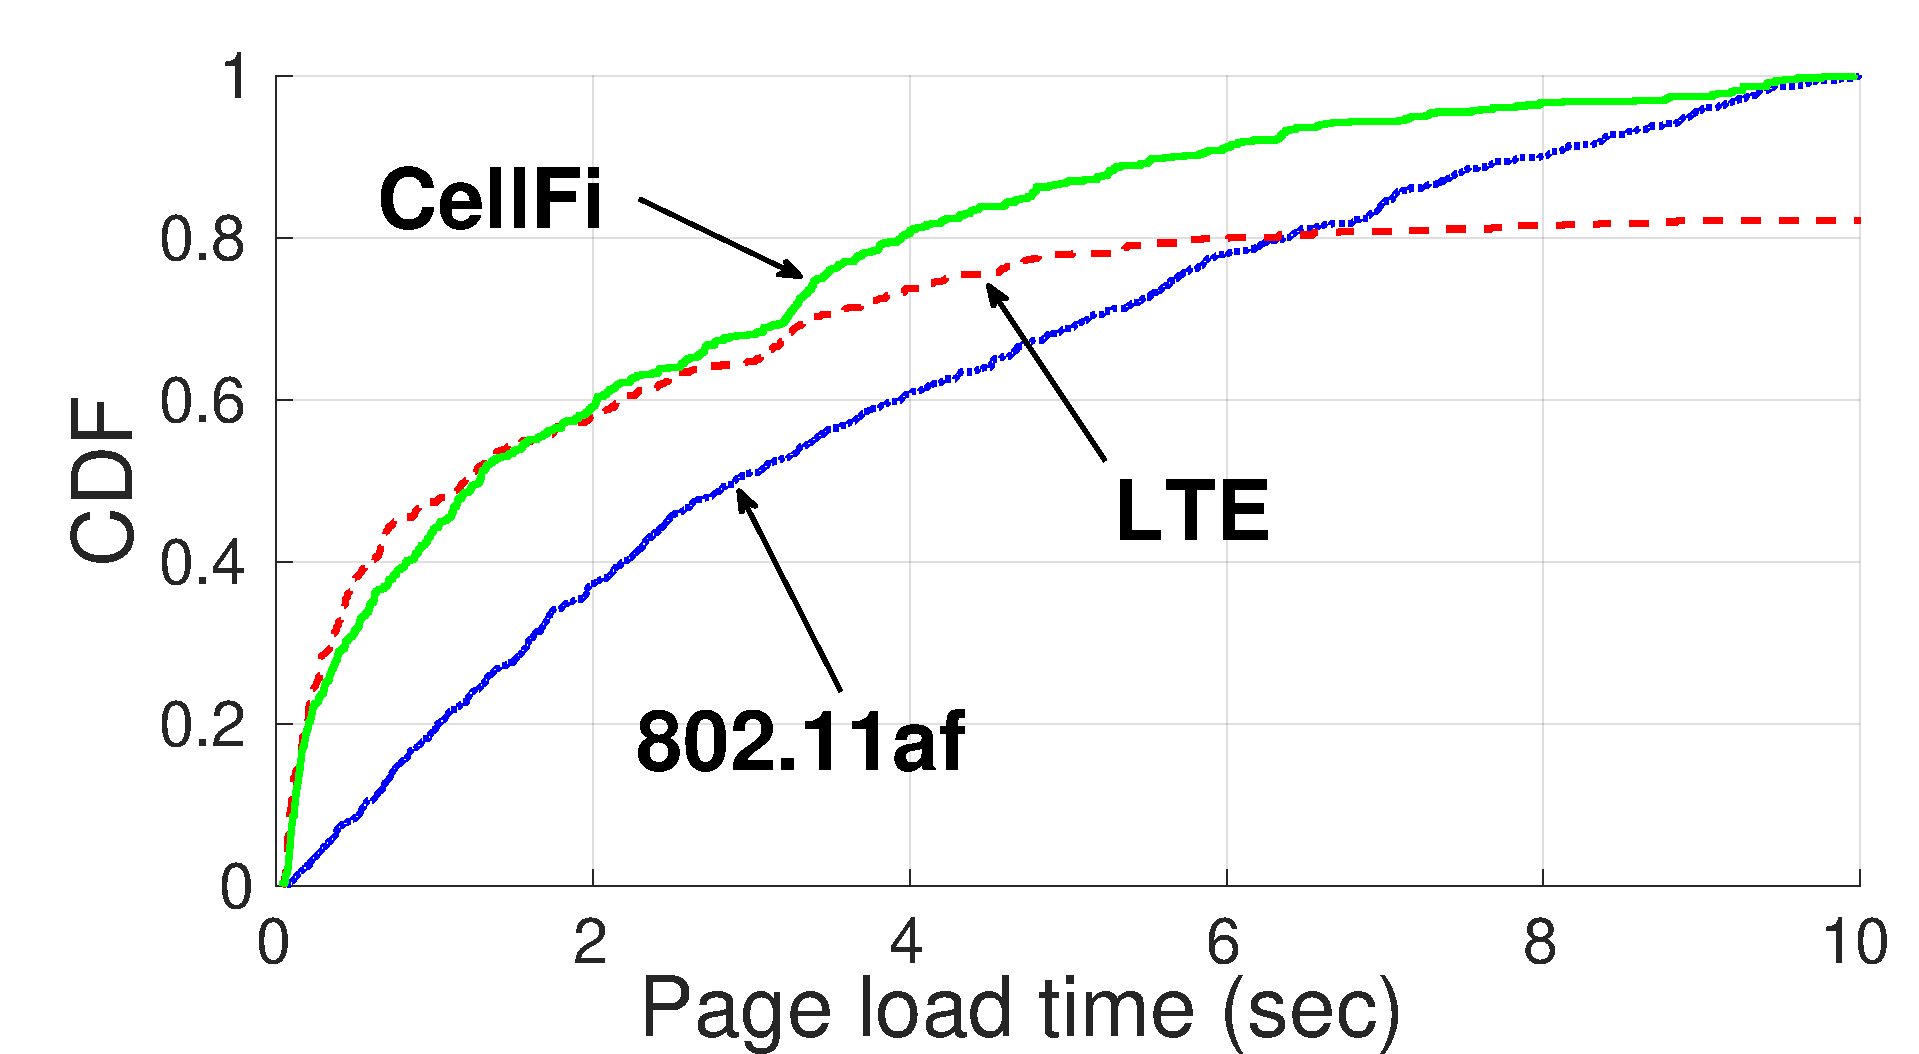
\includegraphics[width=\textwidth]{./figs/FCT-crop}
  \end{minipage}
  \hfill
\vskip -6pt
  \caption{Coverage vs density for \cf, \wf and LTE for 6 clients (a), 
    client throughput of \cf, \wf, LTE and the oracle (b), 
    page load times of \cf, LTE and \wf (c).}
  \label{fig:simulations}
%\vskip -6pt
\end{figure*}



\noindent{\bf Simulation settings.} 
%\label{sec:simset}
We simulate an area of 2 km x 2km, with a varying network density as controlled by the number of simulated APs. 
Base stations are randomly placed in this area with varying number of clients per AP. 
Unless otherwise noted, every scenario is repeated 20 times on a new topology. 

{\em Workloads.} We consider two types of traffic workloads and focus on downlink traffic. 
First, backlogged flows for all clients are used for throughput measurements. Second, 
we model web-like traffic based on realistic parameters regarding flow size, 
number of objects per page~\cite{trafficmodel} and thinking time distributions~\cite{thinktime}. 


%\begin{itemize}
%\item 802.11 VHT mac rates used, mcs 0 - 8 supported
%\item Ideal rate adaptation 
%\item maximum aggregation threshold used (65KB)
%\item RTS/CTS enabled, very low overhead due to high aggregation (without RTS/CTS results are worse)
%\end{itemize}

{\em \wf parameters.} We simulate 802.11af by adjusting the standard 802.11ac PHY and MAC layer in ns3 to match the 802.11af specs~\cite{Rice_af}. 
%with supported VHT MAC rates. 
Our \wf implementation uses ideal rate adaptation based on the 
receiver's SINR value, and supports MPDU aggregation with maximum possible aggregated frame size of 65 KB. 
RTS/CTS is enabled; its overhead is small due to the large aggregation and \wf performance is better with RTS/CTS.
The channel bandwidth for WiFi is set to be 6 MHz.

{\em LTE parameters.} We use the standard ns3 LTE implementation. For \cf, we added 
control channel interference and CQI detection probabilities, both derived from our measurements (Section~\ref{sec:interfeval}).
We choose 5MHz channel and TDD type 2, configuration 4~\cite{36_211} which grants 7 downlink (7ms) and 2 uplink (2ms) subframes in every 10ms frame.
%, which has similar efficiency compared to WiFi, as discussed in Section~\ref{sec:wifilimitations}. 


{\em RF.} WiFi and LTE support different PHY data rates, yielding different coverages. 
We choose the transmit powers for the two networks that provide the same coverage in isolation, 
in order to focus on MAC-layer efficiency.
For WiFi, TX power of both AP and client is set to be 30 dBm. For LTE, TX power of AP is 30 dBm and client is 20 dBm. 
We model loss propagation and noise floor based on our range measurements (Section~\ref{sec:PHY}).



\vskip 2pt
\noindent{\bf Coverage and throughput.}
We have already shown in Section~\ref{sec:PHY} that the link range can go beyond 1km when there is no interference. 
Here, we examine coverage when interfering cells are present. 
We use the static traffic workload and we compare \cf against \wf (802.11af) and LTE.
We also examine the performance a centralized oracle subchannel allocation~\cite{fermi} can achieve.
This provides the extent of performance loss compared to an optimal offline allocation.

Figure~\ref{fig:simulations}(a) shows how coverage varies as the network densifies. 
\cf improves coverage (number of connected users) 
and reduces the number of starved nodes compared to both \cf and LTE. 
For 6 clients per AP and 14 APs, coverage increases by 37\% and 16\% compared to \wf and LTE respectively. 
In an even denser scenario with 16 clients (not shown due to lack of space), 
\cf still offers coverage to more than 80\% of users, an increase of 32\% and 8\% compared to \wf and LTE. 

We now drill down in more detail and examine the performance offered in the densest of the scenarios with 6 clients of Figure~\ref{fig:simulations}(a).
This reflects 84 concurrent clients in a 5MHz channel; note that a typical 3G macro-cell today supports 32 active clients on the same bandwidth~\cite{quora}. 
Figure~\ref{fig:simulations}(b) presents the CDF of client throughput achieved across 20 runs of the experiment.
We observe that \cf improves the overall coverage and fairness, without sacrificing the total throughput in the network.
On the contrary, while with \wf and LTE some clients enjoy higher throughput, this is at the expense of 30-40\% of starved clients due to 
exposed and hidden terminals in the case of \wf, and lack of interference management in the case of LTE. 
Overall, \cf roughly doubles the total throughput achieved per AP compared to \wf at the median, while 
reducing starved clients by roughly 70\% compared to LTE and \wf. 
We also observe that \cf always provides connectivity to more than 90\% of the clients,
while there are cases were \wf and LTE only provide connectivity to 30\% and 60\% of clients respectively.
Note that \cf presents near optimal performance when compared to 
the oracle subchannel allocation (Figure~\ref{fig:simulations}(b)). 



\noindent{\bf Application-level performance.} 
To understand \cf's impact on real applications, we model dynamic traffic conditions based
on our web workload, and examine web-page download times. 
Figure~\ref{fig:simulations} (c) presents the corresponding CDFs of page completion time. The figure
highlights that \cf reduces completion times by 2.3 times at the median compared to \wf, 
and roughly by 8\% relative to LTE. LTE provides marginally better times at smaller percentiles, however
tail performance is significantly degraded due to interference. We also examined whether the network converges. 
We observe that the vast majority of access points only hop very few times in all of our runs; roughly 
1\%-2\% of access points do not converge due to interference and hop almost continuously. 
We omit these figures due to space limitations.

%In Figure~\ref{fig:fct} (right) we plot the CDF of number of channel hop per AP over all runs, normalized by the highest hop number. 
%We see that there is a small fraction of APs that always hop, which are a few starved nodes. 
%Most of the other nodes converge fairly quickly, which explains the observed performance benefits. 


%XXX add discussion about convergence.

%\begin{figure}[h!]
%  \centering
%    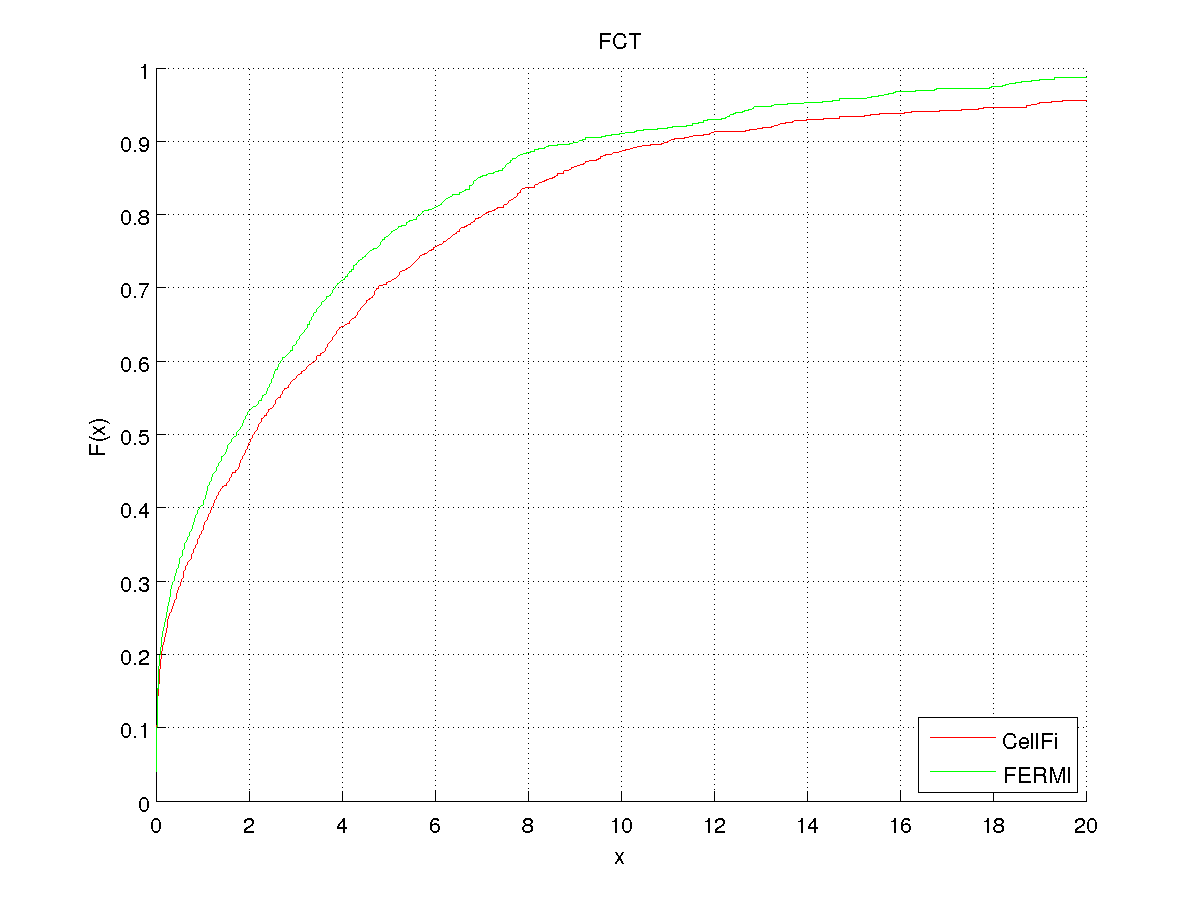
\includegraphics[width=0.5\textwidth]{./figs/FCT-fermi.png}
%  \caption{FCT comparison with FERMI}
%  \label{fct}
%\end{figure}



%\subsubsection{Rate allocations}

%In \ref{minFERMI} and \ref{totalFERMI} we compare CellFi with FERMI~\cite{fermi}. 

%\begin{figure}[t]
%  \centering
%    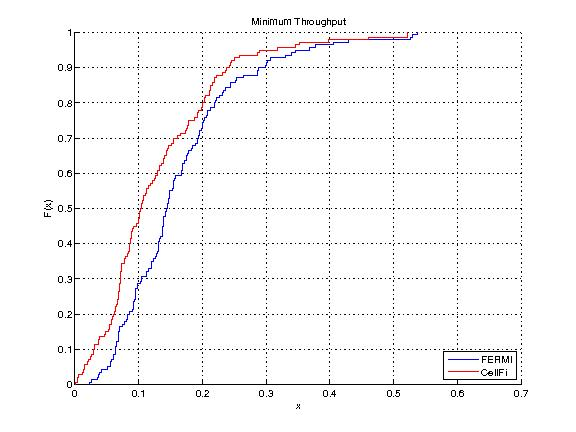
\includegraphics[width=0.45\columnwidth]{./figs/min_CellFi-FERMI.jpg}
%    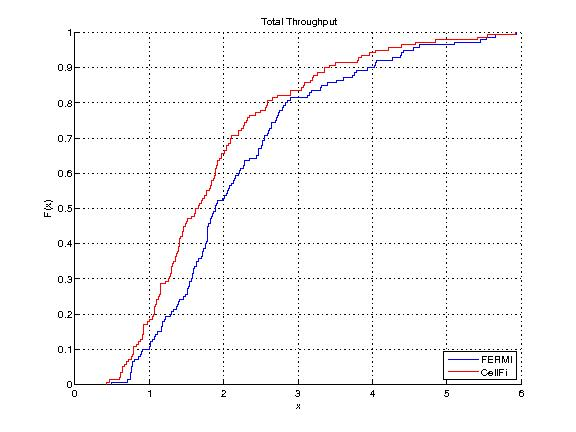
\includegraphics[width=0.45\columnwidth]{./figs/total_CellFi-FERMI.jpg}
%  \caption{Minimum (left) and total (right) throughput of \cf vs the oracle}
%  \label{minFERMI}
%\end{figure}

%\begin{figure}[h!]
%  \centering

%  \caption{Total Throughput Comparison with FERMI}
%  \label{totalFERMI}
%\end{figure}



\noindent{\bf Overheads of signaling.}
CellFi uses mode 3-0 higher layer configured sub-band CQI feedback reports, which consists of 1 wideband CQI value (4 bits) and 13 sub-band CQI values (2 bits). 
The payload size for a single mode 3-0 report on a 5 MHz channel is 20 bits per report. 
The overhead of signaling is 10 Kbps on the uplink for a reporting period of 2 ms. 

%(XXX comment on the overhead) 
